\section{Method}
\label{sec:method}

TaichiDough processes a synchronized RGB-D and motion-capture recording in four stages: metric scene reconstruction, rigid-tool replay, MLS-MPM simulation, and partial-view parameter fitting. Figure~\ref{fig:pipeline} summarizes this sequence. The experimental setup is described first, followed by the simulator and optimization objective.

\subsection{Experimental Setup and Data Collection}

\begin{figure}[t]
    \centering
    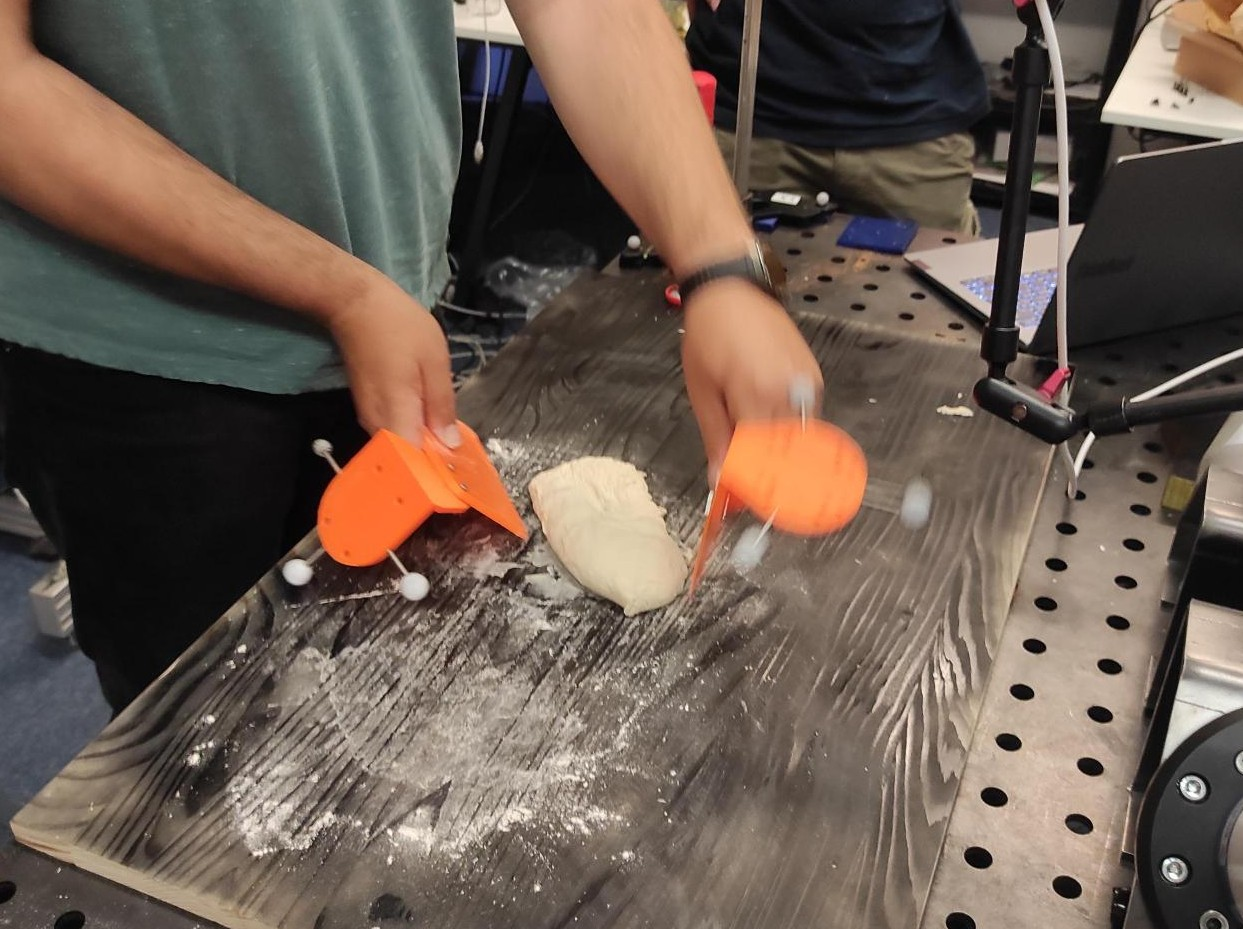
\includegraphics[width=\columnwidth]{figures/data_collection.jpeg}
    \caption{Manual data collection with two 3D-printed spatulas. OptiTrack markers are mounted on the spatulas, while the RGB-D camera observes the dough and tools.}
    \label{fig:data_collection}
\end{figure}

A human operator shaped one dough specimen using two 3D-printed spatulas, as shown in Fig.~\ref{fig:data_collection}. An Intel RealSense D435 recorded aligned color and depth, and an OptiTrack motion-capture system recorded the rigid marker poses attached to both tools. Camera and motion-capture samples were associated by their recorded timestamps. A fixed rigid transform between each marker frame and its registered collision mesh was determined offline and then held constant throughout a replay.

\begin{figure*}[t]
\centering

\includegraphics[width=0.98\textwidth]{matched_sequence.pdf}
\caption{Recorded RGB views and simulated dough-only depth from a separate strictly evaluated Episode~18 run at matched timestamps. The 0.00\,s frame is the initial state; 1.00 and 2.00\,s belong to its fitting interval, while 2.50 and 3.24\,s are later frames of the same replay. The simulator uses the calibrated camera and display crop but does not render spatula occlusion. The later frames are temporal continuation, not an independent test trajectory.}
\label{fig:matched}
\end{figure*}

Let $z_t$ denote the simulated particle state, $u_t$ the recorded poses and pose-derived velocities of the two spatulas, $\theta$ the fitted material variables, and $\psi$ the fixed reconstruction, contact, camera, and numerical settings. For grid spacing $\Delta x$, time step $\Delta t$, and calibrated camera $\mathcal{C}$, the trajectory-conditioned inverse problem is
\begin{equation}
\begin{aligned}
z_{t+1} &= \mathcal{S}_{\Delta x,\Delta t}(z_t,u_t;\theta,\psi),\\
y_t &= \mathcal{H}_{\mathcal{C}}(z_t)+\delta_t+\epsilon_t,
\end{aligned}
\label{eq:inverse_problem}
\end{equation}
where $\mathcal{H}_{\mathcal{C}}$ projects particles into the calibrated depth camera, while $\delta_t$ and $\epsilon_t$ denote model discrepancy and measurement noise. The fitted values are consequently effective parameters of this experiment and simulator rather than direct rheological measurements.

\subsection{Metric Reconstruction and Tool Replay}

Camera intrinsics and a rigid camera-to-motion-capture transform are obtained from repeated AprilTag/motion-capture correspondences. A second fixed rigid transform aligns the measured table plane with the horizontal scene plane. Every point cloud, tool pose, and camera pose is expressed in this metric table-aligned frame; no scale, translation, or post-hoc rigid registration is fitted during evaluation.

The first observed dough surface is voxelized, and each occupied vertical column is filled down to the calibrated table. For reconstructed volume $V$, fixed density $\rho$, and $N$ material points,
\begin{equation}
 M=\rho V,\qquad V_p=V/N,\qquad m_p=\rho V/N.
 \label{eq:mass_initialization}
\end{equation}
The preliminary history run uses $\rho=1200\,\mathrm{kg\,m^{-3}}$, while the separate run visualized in Fig.~\ref{fig:matched} uses $\rho=2196.219\,\mathrm{kg\,m^{-3}}$; density is fixed within each configuration. This construction preserves the represented volume and derived mass when the particle count changes.

Tool positions are linearly interpolated, while quaternion samples are sign-aligned, interpolated, and normalized. Each spatula is represented by a signed-distance field generated from its registered collision mesh. Its velocity at contact point $x$ is
\begin{equation}
 v_{\mathrm{tool}}(x)=v_{\mathrm{lin}}+\omega\times(x-x_c),
 \label{eq:tool_velocity}
\end{equation}
where $x_c$ is the tool center. The implemented unilateral contact update removes inward normal relative velocity and limits tangential correction using the configured Coulomb-friction coefficient; separating motion is unchanged, following the common sticking/sliding/separating treatment used in MPM contact \cite{stomakhin2013snow}.

\subsection{Differentiable MLS-MPM}

The simulator implements three-dimensional MLS-MPM with APIC transfer \cite{hu2018mlsmpm,jiang2015apic} in Taichi \cite{hu2019taichi}. Each particle stores position $x_p$, velocity $v_p$, deformation gradient $F_p$, and affine velocity matrix $C_p$. A trial deformation is first computed as
\begin{equation}
 F_p^*=(I+\Delta t\,C_p^n)F_p^n=U\Sigma V^T,
 \label{eq:deformation_trial}
\end{equation}
where $U$ and $V$ contain the left and right singular vectors and $\Sigma=\operatorname{diag}(\sigma_1,\sigma_2,\sigma_3)$ contains the principal stretches. In the preliminary five-parameter configuration, each stretch is projected according to
\begin{equation}
 \tilde\sigma_i=\operatorname{clip}(\sigma_i,\sigma_{\min},\sigma_{\max}),\qquad
 F_p^{n+1}=U\operatorname{diag}(\tilde\sigma_i)V^T.
 \label{eq:stretch_projection}
\end{equation}
Thus $\sigma_{\min}$ and $\sigma_{\max}$ are dimensionless stretch limits, not yield stresses.

Young's modulus $E$ and Poisson ratio $\nu$ define the Lam\'e parameters
\begin{equation}
 \mu=\frac{E}{2(1+\nu)},\qquad
 \lambda=\frac{E\nu}{(1+\nu)(1-2\nu)}.
 \label{eq:lame}
\end{equation}
With polar factor $R$, $J=\det(F_p)$, and viscosity $\eta$, the implemented Kirchhoff stress contribution is
\begin{equation}
 \tau=2\mu(F_p-R)F_p^T+\lambda J(J-1)I+\eta(C_p+C_p^T).
 \label{eq:stress}
\end{equation}
The final term is an additive rate stress rather than a multi-time-scale rheological model. For quadratic B-spline weight $w_{pi}$, particle-to-node offset $d_{pi}$, grid spacing $\Delta x$, particle volume $V_p$, and particle mass $m_p$, particle-to-grid transfer accumulates
\begin{align}
 m_i &\mathrel{+}=w_{pi}m_p,\\
 m_i v_i &\mathrel{+}=w_{pi}\!\left[m_pv_p+
 \left(-4\Delta t\,V_p\Delta x^{-2}\tau+m_pC_p\right)d_{pi}\right].
 \label{eq:p2g}
\end{align}
The grid-to-particle update reconstructs velocity and affine motion as
\begin{equation}
 v_p^{n+1}=\sum_i w_{pi}v_i,\qquad
 C_p^{n+1}=4\Delta x^{-2}\sum_i w_{pi}v_i d_{pi}^{T}.
 \label{eq:g2p}
\end{equation}

\subsection{Partial-View Objective and Optimization}

At selected frames, a differentiable camera-space particle renderer uses compact splats and soft visibility to produce depth, coverage, and visible particle coordinates. The trajectory objective averages
\begin{equation}
 \mathcal{L}=\frac{1}{|\mathcal{T}|}\sum_{t\in\mathcal{T}}
 \left(0.5\ell_d^t+0.25\ell_c^t+0.25\ell_q^t\right),
 \label{eq:training_loss}
\end{equation}
where $\ell_d$ applies a coverage-blended robust depth-change residual on valid fixed-support pixels and uses a normalized missing-depth residual of $4.0$ where predicted support is absent, $\ell_c$ penalizes missing positive observed foreground, and $\ell_q$ is the directed distance from observed points to visible predicted particles. Measured depth residuals and point distances use a $0.01\,$m scale before the robust penalty. Invalid or unobserved camera pixels are masked out rather than interpreted as measured free space.

Checkpointed reverse-mode differentiation computes gradients of the trajectory loss while bounding device memory. Physical variables are represented by bounded, scaled optimizer coordinates; Young's modulus uses a logarithmic coordinate because of its broad admissible range. A bound-constrained optimizer with backtracking rejects invalid or non-decreasing trial steps. The preliminary run fits $E$, $\nu$, $\eta$, $\sigma_{\min}$, and $\sigma_{\max}$ jointly. Its checkpoint recomputation permits small state and contact-summary mismatches, so the resulting gradients are treated as approximate optimization evidence rather than qualified exact full-trajectory derivatives.
